% Created by tikzDevice version 0.10.1 on 2016-09-01 14:13:40
% !TEX encoding = UTF-8 Unicode
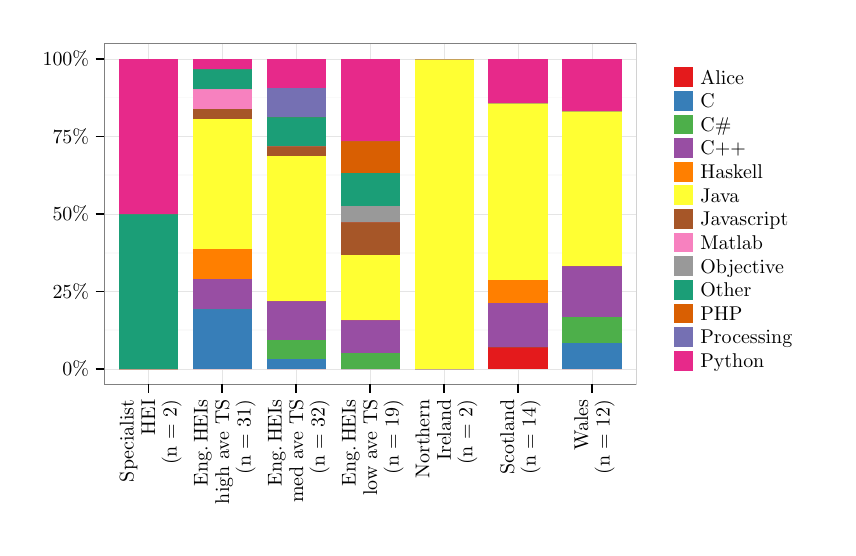
\begin{tikzpicture}[x=1pt,y=1pt]
\definecolor{fillColor}{RGB}{255,255,255}
\path[use as bounding box,fill=fillColor,fill opacity=0.00] (0,0) rectangle (289.08,180.67);
\begin{scope}
\path[clip] (  0.00,  0.00) rectangle (289.08,180.67);
\definecolor{drawColor}{RGB}{255,255,255}
\definecolor{fillColor}{RGB}{255,255,255}

\path[draw=drawColor,line width= 0.6pt,line join=round,line cap=round,fill=fillColor] (  0.00,  0.00) rectangle (289.08,180.68);
\end{scope}
\begin{scope}
\path[clip] ( 27.58, 51.73) rectangle (219.94,174.98);
\definecolor{fillColor}{RGB}{255,255,255}

\path[fill=fillColor] ( 27.58, 51.73) rectangle (219.94,174.98);
\definecolor{drawColor}{gray}{0.98}

\path[draw=drawColor,line width= 0.6pt,line join=round] ( 27.58, 71.34) --
	(219.94, 71.34);

\path[draw=drawColor,line width= 0.6pt,line join=round] ( 27.58, 99.35) --
	(219.94, 99.35);

\path[draw=drawColor,line width= 0.6pt,line join=round] ( 27.58,127.36) --
	(219.94,127.36);

\path[draw=drawColor,line width= 0.6pt,line join=round] ( 27.58,155.38) --
	(219.94,155.38);
\definecolor{drawColor}{gray}{0.90}

\path[draw=drawColor,line width= 0.2pt,line join=round] ( 27.58, 57.33) --
	(219.94, 57.33);

\path[draw=drawColor,line width= 0.2pt,line join=round] ( 27.58, 85.34) --
	(219.94, 85.34);

\path[draw=drawColor,line width= 0.2pt,line join=round] ( 27.58,113.36) --
	(219.94,113.36);

\path[draw=drawColor,line width= 0.2pt,line join=round] ( 27.58,141.37) --
	(219.94,141.37);

\path[draw=drawColor,line width= 0.2pt,line join=round] ( 27.58,169.38) --
	(219.94,169.38);

\path[draw=drawColor,line width= 0.2pt,line join=round] ( 43.61, 51.73) --
	( 43.61,174.98);

\path[draw=drawColor,line width= 0.2pt,line join=round] ( 70.33, 51.73) --
	( 70.33,174.98);

\path[draw=drawColor,line width= 0.2pt,line join=round] ( 97.04, 51.73) --
	( 97.04,174.98);

\path[draw=drawColor,line width= 0.2pt,line join=round] (123.76, 51.73) --
	(123.76,174.98);

\path[draw=drawColor,line width= 0.2pt,line join=round] (150.47, 51.73) --
	(150.47,174.98);

\path[draw=drawColor,line width= 0.2pt,line join=round] (177.19, 51.73) --
	(177.19,174.98);

\path[draw=drawColor,line width= 0.2pt,line join=round] (203.91, 51.73) --
	(203.91,174.98);
\definecolor{fillColor}{RGB}{228,26,28}

\path[fill=fillColor] ( 32.92, 57.33) rectangle ( 54.30, 57.33);
\definecolor{fillColor}{RGB}{55,126,184}

\path[fill=fillColor] ( 32.92, 57.33) rectangle ( 54.30, 57.33);
\definecolor{fillColor}{RGB}{77,175,74}

\path[fill=fillColor] ( 32.92, 57.33) rectangle ( 54.30, 57.33);
\definecolor{fillColor}{RGB}{152,78,163}

\path[fill=fillColor] ( 32.92, 57.33) rectangle ( 54.30, 57.33);
\definecolor{fillColor}{RGB}{255,127,0}

\path[fill=fillColor] ( 32.92, 57.33) rectangle ( 54.30, 57.33);
\definecolor{fillColor}{RGB}{255,255,51}

\path[fill=fillColor] ( 32.92, 57.33) rectangle ( 54.30, 57.33);
\definecolor{fillColor}{RGB}{166,86,40}

\path[fill=fillColor] ( 32.92, 57.33) rectangle ( 54.30, 57.33);
\definecolor{fillColor}{RGB}{247,129,191}

\path[fill=fillColor] ( 32.92, 57.33) rectangle ( 54.30, 57.33);
\definecolor{fillColor}{gray}{0.60}

\path[fill=fillColor] ( 32.92, 57.33) rectangle ( 54.30, 57.33);
\definecolor{fillColor}{RGB}{27,158,119}

\path[fill=fillColor] ( 32.92, 57.33) rectangle ( 54.30,113.36);
\definecolor{fillColor}{RGB}{217,95,2}

\path[fill=fillColor] ( 32.92,113.36) rectangle ( 54.30,113.36);
\definecolor{fillColor}{RGB}{117,112,179}

\path[fill=fillColor] ( 32.92,113.36) rectangle ( 54.30,113.36);
\definecolor{fillColor}{RGB}{231,41,138}

\path[fill=fillColor] ( 32.92,113.36) rectangle ( 54.30,169.38);
\definecolor{fillColor}{RGB}{228,26,28}

\path[fill=fillColor] ( 59.64, 57.33) rectangle ( 81.01, 57.33);
\definecolor{fillColor}{RGB}{55,126,184}

\path[fill=fillColor] ( 59.64, 57.33) rectangle ( 81.01, 79.02);
\definecolor{fillColor}{RGB}{77,175,74}

\path[fill=fillColor] ( 59.64, 79.02) rectangle ( 81.01, 79.02);
\definecolor{fillColor}{RGB}{152,78,163}

\path[fill=fillColor] ( 59.64, 79.02) rectangle ( 81.01, 89.86);
\definecolor{fillColor}{RGB}{255,127,0}

\path[fill=fillColor] ( 59.64, 89.86) rectangle ( 81.01,100.70);
\definecolor{fillColor}{RGB}{255,255,51}

\path[fill=fillColor] ( 59.64,100.70) rectangle ( 81.01,147.69);
\definecolor{fillColor}{RGB}{166,86,40}

\path[fill=fillColor] ( 59.64,147.69) rectangle ( 81.01,151.31);
\definecolor{fillColor}{RGB}{247,129,191}

\path[fill=fillColor] ( 59.64,151.31) rectangle ( 81.01,158.54);
\definecolor{fillColor}{gray}{0.60}

\path[fill=fillColor] ( 59.64,158.54) rectangle ( 81.01,158.54);
\definecolor{fillColor}{RGB}{27,158,119}

\path[fill=fillColor] ( 59.64,158.54) rectangle ( 81.01,165.77);
\definecolor{fillColor}{RGB}{217,95,2}

\path[fill=fillColor] ( 59.64,165.77) rectangle ( 81.01,165.77);
\definecolor{fillColor}{RGB}{117,112,179}

\path[fill=fillColor] ( 59.64,165.77) rectangle ( 81.01,165.77);
\definecolor{fillColor}{RGB}{231,41,138}

\path[fill=fillColor] ( 59.64,165.77) rectangle ( 81.01,169.38);
\definecolor{fillColor}{RGB}{228,26,28}

\path[fill=fillColor] ( 86.36, 57.33) rectangle (107.73, 57.33);
\definecolor{fillColor}{RGB}{55,126,184}

\path[fill=fillColor] ( 86.36, 57.33) rectangle (107.73, 60.83);
\definecolor{fillColor}{RGB}{77,175,74}

\path[fill=fillColor] ( 86.36, 60.83) rectangle (107.73, 67.83);
\definecolor{fillColor}{RGB}{152,78,163}

\path[fill=fillColor] ( 86.36, 67.83) rectangle (107.73, 81.84);
\definecolor{fillColor}{RGB}{255,127,0}

\path[fill=fillColor] ( 86.36, 81.84) rectangle (107.73, 81.84);
\definecolor{fillColor}{RGB}{255,255,51}

\path[fill=fillColor] ( 86.36, 81.84) rectangle (107.73,134.37);
\definecolor{fillColor}{RGB}{166,86,40}

\path[fill=fillColor] ( 86.36,134.37) rectangle (107.73,137.87);
\definecolor{fillColor}{RGB}{247,129,191}

\path[fill=fillColor] ( 86.36,137.87) rectangle (107.73,137.87);
\definecolor{fillColor}{gray}{0.60}

\path[fill=fillColor] ( 86.36,137.87) rectangle (107.73,137.87);
\definecolor{fillColor}{RGB}{27,158,119}

\path[fill=fillColor] ( 86.36,137.87) rectangle (107.73,148.37);
\definecolor{fillColor}{RGB}{217,95,2}

\path[fill=fillColor] ( 86.36,148.37) rectangle (107.73,148.37);
\definecolor{fillColor}{RGB}{117,112,179}

\path[fill=fillColor] ( 86.36,148.37) rectangle (107.73,158.88);
\definecolor{fillColor}{RGB}{231,41,138}

\path[fill=fillColor] ( 86.36,158.88) rectangle (107.73,169.38);
\definecolor{fillColor}{RGB}{228,26,28}

\path[fill=fillColor] (113.07, 57.33) rectangle (134.44, 57.33);
\definecolor{fillColor}{RGB}{55,126,184}

\path[fill=fillColor] (113.07, 57.33) rectangle (134.44, 57.33);
\definecolor{fillColor}{RGB}{77,175,74}

\path[fill=fillColor] (113.07, 57.33) rectangle (134.44, 63.23);
\definecolor{fillColor}{RGB}{152,78,163}

\path[fill=fillColor] (113.07, 63.23) rectangle (134.44, 75.02);
\definecolor{fillColor}{RGB}{255,127,0}

\path[fill=fillColor] (113.07, 75.02) rectangle (134.44, 75.02);
\definecolor{fillColor}{RGB}{255,255,51}

\path[fill=fillColor] (113.07, 75.02) rectangle (134.44, 98.61);
\definecolor{fillColor}{RGB}{166,86,40}

\path[fill=fillColor] (113.07, 98.61) rectangle (134.44,110.41);
\definecolor{fillColor}{RGB}{247,129,191}

\path[fill=fillColor] (113.07,110.41) rectangle (134.44,110.41);
\definecolor{fillColor}{gray}{0.60}

\path[fill=fillColor] (113.07,110.41) rectangle (134.44,116.30);
\definecolor{fillColor}{RGB}{27,158,119}

\path[fill=fillColor] (113.07,116.30) rectangle (134.44,128.10);
\definecolor{fillColor}{RGB}{217,95,2}

\path[fill=fillColor] (113.07,128.10) rectangle (134.44,139.89);
\definecolor{fillColor}{RGB}{117,112,179}

\path[fill=fillColor] (113.07,139.89) rectangle (134.44,139.89);
\definecolor{fillColor}{RGB}{231,41,138}

\path[fill=fillColor] (113.07,139.89) rectangle (134.44,169.38);
\definecolor{fillColor}{RGB}{228,26,28}

\path[fill=fillColor] (139.79, 57.33) rectangle (161.16, 57.33);
\definecolor{fillColor}{RGB}{55,126,184}

\path[fill=fillColor] (139.79, 57.33) rectangle (161.16, 57.33);
\definecolor{fillColor}{RGB}{77,175,74}

\path[fill=fillColor] (139.79, 57.33) rectangle (161.16, 57.33);
\definecolor{fillColor}{RGB}{152,78,163}

\path[fill=fillColor] (139.79, 57.33) rectangle (161.16, 57.33);
\definecolor{fillColor}{RGB}{255,127,0}

\path[fill=fillColor] (139.79, 57.33) rectangle (161.16, 57.33);
\definecolor{fillColor}{RGB}{255,255,51}

\path[fill=fillColor] (139.79, 57.33) rectangle (161.16,169.38);
\definecolor{fillColor}{RGB}{166,86,40}

\path[fill=fillColor] (139.79,169.38) rectangle (161.16,169.38);
\definecolor{fillColor}{RGB}{247,129,191}

\path[fill=fillColor] (139.79,169.38) rectangle (161.16,169.38);
\definecolor{fillColor}{gray}{0.60}

\path[fill=fillColor] (139.79,169.38) rectangle (161.16,169.38);
\definecolor{fillColor}{RGB}{27,158,119}

\path[fill=fillColor] (139.79,169.38) rectangle (161.16,169.38);
\definecolor{fillColor}{RGB}{217,95,2}

\path[fill=fillColor] (139.79,169.38) rectangle (161.16,169.38);
\definecolor{fillColor}{RGB}{117,112,179}

\path[fill=fillColor] (139.79,169.38) rectangle (161.16,169.38);
\definecolor{fillColor}{RGB}{231,41,138}

\path[fill=fillColor] (139.79,169.38) rectangle (161.16,169.38);
\definecolor{fillColor}{RGB}{228,26,28}

\path[fill=fillColor] (166.50, 57.33) rectangle (187.88, 65.33);
\definecolor{fillColor}{RGB}{55,126,184}

\path[fill=fillColor] (166.50, 65.33) rectangle (187.88, 65.33);
\definecolor{fillColor}{RGB}{77,175,74}

\path[fill=fillColor] (166.50, 65.33) rectangle (187.88, 65.33);
\definecolor{fillColor}{RGB}{152,78,163}

\path[fill=fillColor] (166.50, 65.33) rectangle (187.88, 81.34);
\definecolor{fillColor}{RGB}{255,127,0}

\path[fill=fillColor] (166.50, 81.34) rectangle (187.88, 89.34);
\definecolor{fillColor}{RGB}{255,255,51}

\path[fill=fillColor] (166.50, 89.34) rectangle (187.88,153.37);
\definecolor{fillColor}{RGB}{166,86,40}

\path[fill=fillColor] (166.50,153.37) rectangle (187.88,153.37);
\definecolor{fillColor}{RGB}{247,129,191}

\path[fill=fillColor] (166.50,153.37) rectangle (187.88,153.37);
\definecolor{fillColor}{gray}{0.60}

\path[fill=fillColor] (166.50,153.37) rectangle (187.88,153.37);
\definecolor{fillColor}{RGB}{27,158,119}

\path[fill=fillColor] (166.50,153.37) rectangle (187.88,153.37);
\definecolor{fillColor}{RGB}{217,95,2}

\path[fill=fillColor] (166.50,153.37) rectangle (187.88,153.37);
\definecolor{fillColor}{RGB}{117,112,179}

\path[fill=fillColor] (166.50,153.37) rectangle (187.88,153.37);
\definecolor{fillColor}{RGB}{231,41,138}

\path[fill=fillColor] (166.50,153.37) rectangle (187.88,169.38);
\definecolor{fillColor}{RGB}{228,26,28}

\path[fill=fillColor] (193.22, 57.33) rectangle (214.59, 57.33);
\definecolor{fillColor}{RGB}{55,126,184}

\path[fill=fillColor] (193.22, 57.33) rectangle (214.59, 66.67);
\definecolor{fillColor}{RGB}{77,175,74}

\path[fill=fillColor] (193.22, 66.67) rectangle (214.59, 76.00);
\definecolor{fillColor}{RGB}{152,78,163}

\path[fill=fillColor] (193.22, 76.00) rectangle (214.59, 94.68);
\definecolor{fillColor}{RGB}{255,127,0}

\path[fill=fillColor] (193.22, 94.68) rectangle (214.59, 94.68);
\definecolor{fillColor}{RGB}{255,255,51}

\path[fill=fillColor] (193.22, 94.68) rectangle (214.59,150.71);
\definecolor{fillColor}{RGB}{166,86,40}

\path[fill=fillColor] (193.22,150.71) rectangle (214.59,150.71);
\definecolor{fillColor}{RGB}{247,129,191}

\path[fill=fillColor] (193.22,150.71) rectangle (214.59,150.71);
\definecolor{fillColor}{gray}{0.60}

\path[fill=fillColor] (193.22,150.71) rectangle (214.59,150.71);
\definecolor{fillColor}{RGB}{27,158,119}

\path[fill=fillColor] (193.22,150.71) rectangle (214.59,150.71);
\definecolor{fillColor}{RGB}{217,95,2}

\path[fill=fillColor] (193.22,150.71) rectangle (214.59,150.71);
\definecolor{fillColor}{RGB}{117,112,179}

\path[fill=fillColor] (193.22,150.71) rectangle (214.59,150.71);
\definecolor{fillColor}{RGB}{231,41,138}

\path[fill=fillColor] (193.22,150.71) rectangle (214.59,169.38);
\definecolor{drawColor}{gray}{0.50}

\path[draw=drawColor,line width= 0.6pt,line join=round,line cap=round] ( 27.58, 51.73) rectangle (219.94,174.98);
\end{scope}
\begin{scope}
\path[clip] (  0.00,  0.00) rectangle (289.08,180.67);
\definecolor{drawColor}{RGB}{0,0,0}

\node[text=drawColor,anchor=base east,inner sep=0pt, outer sep=0pt, scale=  0.72] at ( 22.18, 54.85) {0\%};

\node[text=drawColor,anchor=base east,inner sep=0pt, outer sep=0pt, scale=  0.72] at ( 22.18, 82.86) {25\%};

\node[text=drawColor,anchor=base east,inner sep=0pt, outer sep=0pt, scale=  0.72] at ( 22.18,110.88) {50\%};

\node[text=drawColor,anchor=base east,inner sep=0pt, outer sep=0pt, scale=  0.72] at ( 22.18,138.89) {75\%};

\node[text=drawColor,anchor=base east,inner sep=0pt, outer sep=0pt, scale=  0.72] at ( 22.18,166.90) {100\%};
\end{scope}
\begin{scope}
\path[clip] (  0.00,  0.00) rectangle (289.08,180.67);
\definecolor{drawColor}{RGB}{0,0,0}

\path[draw=drawColor,line width= 0.6pt,line join=round] ( 24.58, 57.33) --
	( 27.58, 57.33);

\path[draw=drawColor,line width= 0.6pt,line join=round] ( 24.58, 85.34) --
	( 27.58, 85.34);

\path[draw=drawColor,line width= 0.6pt,line join=round] ( 24.58,113.36) --
	( 27.58,113.36);

\path[draw=drawColor,line width= 0.6pt,line join=round] ( 24.58,141.37) --
	( 27.58,141.37);

\path[draw=drawColor,line width= 0.6pt,line join=round] ( 24.58,169.38) --
	( 27.58,169.38);
\end{scope}
\begin{scope}
\path[clip] (  0.00,  0.00) rectangle (289.08,180.67);
\definecolor{drawColor}{RGB}{0,0,0}

\path[draw=drawColor,line width= 0.6pt,line join=round] ( 43.61, 48.73) --
	( 43.61, 51.73);

\path[draw=drawColor,line width= 0.6pt,line join=round] ( 70.33, 48.73) --
	( 70.33, 51.73);

\path[draw=drawColor,line width= 0.6pt,line join=round] ( 97.04, 48.73) --
	( 97.04, 51.73);

\path[draw=drawColor,line width= 0.6pt,line join=round] (123.76, 48.73) --
	(123.76, 51.73);

\path[draw=drawColor,line width= 0.6pt,line join=round] (150.47, 48.73) --
	(150.47, 51.73);

\path[draw=drawColor,line width= 0.6pt,line join=round] (177.19, 48.73) --
	(177.19, 51.73);

\path[draw=drawColor,line width= 0.6pt,line join=round] (203.91, 48.73) --
	(203.91, 51.73);
\end{scope}
\begin{scope}
\path[clip] (  0.00,  0.00) rectangle (289.08,180.67);
\definecolor{drawColor}{RGB}{0,0,0}

\node[text=drawColor,rotate= 90.00,anchor=base east,inner sep=0pt, outer sep=0pt, scale=  0.72] at ( 38.31, 46.33) {Specialist};

\node[text=drawColor,rotate= 90.00,anchor=base east,inner sep=0pt, outer sep=0pt, scale=  0.72] at ( 46.09, 46.33) {HEI};

\node[text=drawColor,rotate= 90.00,anchor=base east,inner sep=0pt, outer sep=0pt, scale=  0.72] at ( 53.86, 46.33) {(n = 2)};

\node[text=drawColor,rotate= 90.00,anchor=base east,inner sep=0pt, outer sep=0pt, scale=  0.72] at ( 65.03, 46.33) {Eng.\,HEIs};

\node[text=drawColor,rotate= 90.00,anchor=base east,inner sep=0pt, outer sep=0pt, scale=  0.72] at ( 72.80, 46.33) {high ave TS};

\node[text=drawColor,rotate= 90.00,anchor=base east,inner sep=0pt, outer sep=0pt, scale=  0.72] at ( 80.58, 46.33) {(n = 31)};

\node[text=drawColor,rotate= 90.00,anchor=base east,inner sep=0pt, outer sep=0pt, scale=  0.72] at ( 91.75, 46.33) {Eng.\,HEIs};

\node[text=drawColor,rotate= 90.00,anchor=base east,inner sep=0pt, outer sep=0pt, scale=  0.72] at ( 99.52, 46.33) {med ave TS};

\node[text=drawColor,rotate= 90.00,anchor=base east,inner sep=0pt, outer sep=0pt, scale=  0.72] at (107.30, 46.33) {(n = 32)};

\node[text=drawColor,rotate= 90.00,anchor=base east,inner sep=0pt, outer sep=0pt, scale=  0.72] at (118.46, 46.33) {Eng.\,HEIs};

\node[text=drawColor,rotate= 90.00,anchor=base east,inner sep=0pt, outer sep=0pt, scale=  0.72] at (126.24, 46.33) {low ave TS};

\node[text=drawColor,rotate= 90.00,anchor=base east,inner sep=0pt, outer sep=0pt, scale=  0.72] at (134.01, 46.33) {(n = 19)};

\node[text=drawColor,rotate= 90.00,anchor=base east,inner sep=0pt, outer sep=0pt, scale=  0.72] at (145.18, 46.33) {Northern};

\node[text=drawColor,rotate= 90.00,anchor=base east,inner sep=0pt, outer sep=0pt, scale=  0.72] at (152.95, 46.33) {Ireland};

\node[text=drawColor,rotate= 90.00,anchor=base east,inner sep=0pt, outer sep=0pt, scale=  0.72] at (160.73, 46.33) {(n = 2)};

\node[text=drawColor,rotate= 90.00,anchor=base east,inner sep=0pt, outer sep=0pt, scale=  0.72] at (175.78, 46.33) {Scotland};

\node[text=drawColor,rotate= 90.00,anchor=base east,inner sep=0pt, outer sep=0pt, scale=  0.72] at (183.56, 46.33) {(n = 14)};

\node[text=drawColor,rotate= 90.00,anchor=base east,inner sep=0pt, outer sep=0pt, scale=  0.72] at (202.50, 46.33) {Wales};

\node[text=drawColor,rotate= 90.00,anchor=base east,inner sep=0pt, outer sep=0pt, scale=  0.72] at (210.28, 46.33) {(n = 12)};
\end{scope}
\begin{scope}
\path[clip] (  0.00,  0.00) rectangle (289.08,180.67);
\definecolor{fillColor}{RGB}{255,255,255}

\path[fill=fillColor] (228.47, 51.80) rectangle (280.54,174.91);
\end{scope}
\begin{scope}
\path[clip] (  0.00,  0.00) rectangle (289.08,180.67);
\definecolor{fillColor}{RGB}{228,26,28}

\path[fill=fillColor] (233.45,159.21) rectangle (240.57,166.32);
\end{scope}
\begin{scope}
\path[clip] (  0.00,  0.00) rectangle (289.08,180.67);
\definecolor{fillColor}{RGB}{55,126,184}

\path[fill=fillColor] (233.45,150.67) rectangle (240.57,157.78);
\end{scope}
\begin{scope}
\path[clip] (  0.00,  0.00) rectangle (289.08,180.67);
\definecolor{fillColor}{RGB}{77,175,74}

\path[fill=fillColor] (233.45,142.14) rectangle (240.57,149.25);
\end{scope}
\begin{scope}
\path[clip] (  0.00,  0.00) rectangle (289.08,180.67);
\definecolor{fillColor}{RGB}{152,78,163}

\path[fill=fillColor] (233.45,133.60) rectangle (240.57,140.71);
\end{scope}
\begin{scope}
\path[clip] (  0.00,  0.00) rectangle (289.08,180.67);
\definecolor{fillColor}{RGB}{255,127,0}

\path[fill=fillColor] (233.45,125.06) rectangle (240.57,132.18);
\end{scope}
\begin{scope}
\path[clip] (  0.00,  0.00) rectangle (289.08,180.67);
\definecolor{fillColor}{RGB}{255,255,51}

\path[fill=fillColor] (233.45,116.53) rectangle (240.57,123.64);
\end{scope}
\begin{scope}
\path[clip] (  0.00,  0.00) rectangle (289.08,180.67);
\definecolor{fillColor}{RGB}{166,86,40}

\path[fill=fillColor] (233.45,107.99) rectangle (240.57,115.11);
\end{scope}
\begin{scope}
\path[clip] (  0.00,  0.00) rectangle (289.08,180.67);
\definecolor{fillColor}{RGB}{247,129,191}

\path[fill=fillColor] (233.45, 99.46) rectangle (240.57,106.57);
\end{scope}
\begin{scope}
\path[clip] (  0.00,  0.00) rectangle (289.08,180.67);
\definecolor{fillColor}{gray}{0.60}

\path[fill=fillColor] (233.45, 90.92) rectangle (240.57, 98.03);
\end{scope}
\begin{scope}
\path[clip] (  0.00,  0.00) rectangle (289.08,180.67);
\definecolor{fillColor}{RGB}{27,158,119}

\path[fill=fillColor] (233.45, 82.38) rectangle (240.57, 89.50);
\end{scope}
\begin{scope}
\path[clip] (  0.00,  0.00) rectangle (289.08,180.67);
\definecolor{fillColor}{RGB}{217,95,2}

\path[fill=fillColor] (233.45, 73.85) rectangle (240.57, 80.96);
\end{scope}
\begin{scope}
\path[clip] (  0.00,  0.00) rectangle (289.08,180.67);
\definecolor{fillColor}{RGB}{117,112,179}

\path[fill=fillColor] (233.45, 65.31) rectangle (240.57, 72.43);
\end{scope}
\begin{scope}
\path[clip] (  0.00,  0.00) rectangle (289.08,180.67);
\definecolor{fillColor}{RGB}{231,41,138}

\path[fill=fillColor] (233.45, 56.78) rectangle (240.57, 63.89);
\end{scope}
\begin{scope}
\path[clip] (  0.00,  0.00) rectangle (289.08,180.67);
\definecolor{drawColor}{RGB}{0,0,0}

\node[text=drawColor,anchor=base west,inner sep=0pt, outer sep=0pt, scale=  0.72] at (243.08,160.28) {Alice};
\end{scope}
\begin{scope}
\path[clip] (  0.00,  0.00) rectangle (289.08,180.67);
\definecolor{drawColor}{RGB}{0,0,0}

\node[text=drawColor,anchor=base west,inner sep=0pt, outer sep=0pt, scale=  0.72] at (243.08,151.75) {C};
\end{scope}
\begin{scope}
\path[clip] (  0.00,  0.00) rectangle (289.08,180.67);
\definecolor{drawColor}{RGB}{0,0,0}

\node[text=drawColor,anchor=base west,inner sep=0pt, outer sep=0pt, scale=  0.72] at (243.08,143.21) {C\#};
\end{scope}
\begin{scope}
\path[clip] (  0.00,  0.00) rectangle (289.08,180.67);
\definecolor{drawColor}{RGB}{0,0,0}

\node[text=drawColor,anchor=base west,inner sep=0pt, outer sep=0pt, scale=  0.72] at (243.08,134.68) {C++};
\end{scope}
\begin{scope}
\path[clip] (  0.00,  0.00) rectangle (289.08,180.67);
\definecolor{drawColor}{RGB}{0,0,0}

\node[text=drawColor,anchor=base west,inner sep=0pt, outer sep=0pt, scale=  0.72] at (243.08,126.14) {Haskell};
\end{scope}
\begin{scope}
\path[clip] (  0.00,  0.00) rectangle (289.08,180.67);
\definecolor{drawColor}{RGB}{0,0,0}

\node[text=drawColor,anchor=base west,inner sep=0pt, outer sep=0pt, scale=  0.72] at (243.08,117.61) {Java};
\end{scope}
\begin{scope}
\path[clip] (  0.00,  0.00) rectangle (289.08,180.67);
\definecolor{drawColor}{RGB}{0,0,0}

\node[text=drawColor,anchor=base west,inner sep=0pt, outer sep=0pt, scale=  0.72] at (243.08,109.07) {Javascript};
\end{scope}
\begin{scope}
\path[clip] (  0.00,  0.00) rectangle (289.08,180.67);
\definecolor{drawColor}{RGB}{0,0,0}

\node[text=drawColor,anchor=base west,inner sep=0pt, outer sep=0pt, scale=  0.72] at (243.08,100.53) {Matlab};
\end{scope}
\begin{scope}
\path[clip] (  0.00,  0.00) rectangle (289.08,180.67);
\definecolor{drawColor}{RGB}{0,0,0}

\node[text=drawColor,anchor=base west,inner sep=0pt, outer sep=0pt, scale=  0.72] at (243.08, 92.00) {Objective};
\end{scope}
\begin{scope}
\path[clip] (  0.00,  0.00) rectangle (289.08,180.67);
\definecolor{drawColor}{RGB}{0,0,0}

\node[text=drawColor,anchor=base west,inner sep=0pt, outer sep=0pt, scale=  0.72] at (243.08, 83.46) {Other};
\end{scope}
\begin{scope}
\path[clip] (  0.00,  0.00) rectangle (289.08,180.67);
\definecolor{drawColor}{RGB}{0,0,0}

\node[text=drawColor,anchor=base west,inner sep=0pt, outer sep=0pt, scale=  0.72] at (243.08, 74.93) {PHP};
\end{scope}
\begin{scope}
\path[clip] (  0.00,  0.00) rectangle (289.08,180.67);
\definecolor{drawColor}{RGB}{0,0,0}

\node[text=drawColor,anchor=base west,inner sep=0pt, outer sep=0pt, scale=  0.72] at (243.08, 66.39) {Processing};
\end{scope}
\begin{scope}
\path[clip] (  0.00,  0.00) rectangle (289.08,180.67);
\definecolor{drawColor}{RGB}{0,0,0}

\node[text=drawColor,anchor=base west,inner sep=0pt, outer sep=0pt, scale=  0.72] at (243.08, 57.85) {Python};
\end{scope}
\end{tikzpicture}
